\documentclass[12pt]{article}
\usepackage{amsfonts, amsmath, amsthm, amssymb}
\usepackage[left=1cm,right=1cm,top=1cm,bottom=2cm]{geometry}
\usepackage{paralist}
\usepackage[T2A]{fontenc}
\usepackage[russian]{babel}
\usepackage[utf8]{inputenc}
\usepackage{graphicx}
\usepackage{wrapfig}

\usepackage{mathtools}
\usepackage{comment}
\DeclareGraphicsRule{*}{mps}{*}{}

\newcounter{problem}
\newcommand{\problem}{\par \bigskip \refstepcounter{problem}%
\textbf{№\arabic{problem}.} }

\def\avtor#1{\linebreak[2] \hspace*{\fill}{\small (\mbox{\textit{#1})}}}

\def \Problem#1{\par \bigskip \textbf{Задача №{#1}. }}
\def \solution{\par \bigskip \textbf{Решение. }}
\def \solutionI{\par \bigskip \textbf{Первое решение. }}
\def \solutionII{\par \bigskip \textbf{Второе решение. }}
\def \solutionIII{\par \bigskip \textbf{Третье решение. }}
\def \Lemma{\par \bigskip \textbf{Лемма. }}
\def \lemma#1{\par \bigskip \textbf{Лемма {#1}. }}
\def \proof{\par \bigskip \textbf{Доказательство. }}
\def \answer{\par \bigskip \textbf{Ответ. }}
\def \marking{\par \bigskip \textbf{Схема оценки. }}
\def \corollary{\par \bigskip \textbf{Следствие. }}
\def\geq{\geqslant}
\def\leq{\leqslant}
\def\frac#1#2{\mathchoice{#1\over#2}{\hbox{\small$#1$}\over\mathstrut\hbox{\small$#2$}}{#1\over#2}{#1\over#2}} 

\begin{document}
\centerline{\sc \textbf{XXII Математическая олимпиада <<Шелковый путь>>}}

\centerline{\sc \textbf{Март 2023 года}}

\bigskip
\hrule
\bigskip

\textsl{\textbf{Внимание!} 
Так как XXII Математическая олимпиада «Шёлковый путь» проводится в разных странах в разные дни, мы вас убедительно просим \textbf{не разглашать} эти задачи и не обсуждать их (особенно по Интернету) до 25 мая 2023 года.
}

\bigskip

\centerline{\sc \textbf{Решения задач и схемы оценки}}

\bigskip
\Problem{1} Внутри трапеции $ABCD$ $(AD \parallel BC)$  выбрана точка $M$, а внутри треугольника $BMC$ точка $N$ так, что $AM \parallel CN$, $BM \parallel DN$. Докажите, что у треугольников $ABN$ и $CDM$ площади равны. \avtor{Седракян~Н.}

\solution Докажем сначала следующую лемму.

\Lemma На боковых сторонах $XY$ и $ZT$ трапеции $XYZT$ взяты точки $N$ и $M$, соответственно. Известно, что $XM \parallel ZN$. Тогда $YM \parallel TN$.

\proof Так как 
$$
S_{NYZM}= S_{NYZ}+ S_{NZM}= S_{NYZ}+ S_{XNZ}= S_{XYZ} = S_{YZT}= S_{YZM}+ S_{YMT},
$$
то
$$
S_{YZM}+ S_{YMT}= S_{NYZM}= S_{YZM}+ S_{NYM},
$$
а значит $S_{YMT}= S_{NYM}$. Поэтому, $YM \parallel NT$. \qed

$$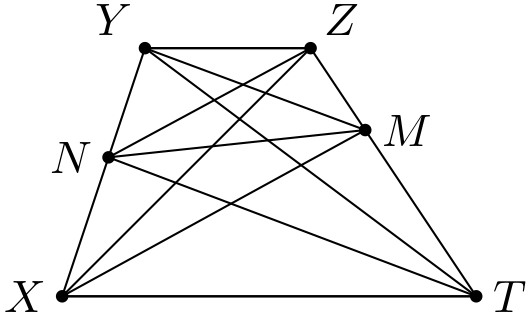
\includegraphics{img_1.jpg} \quad 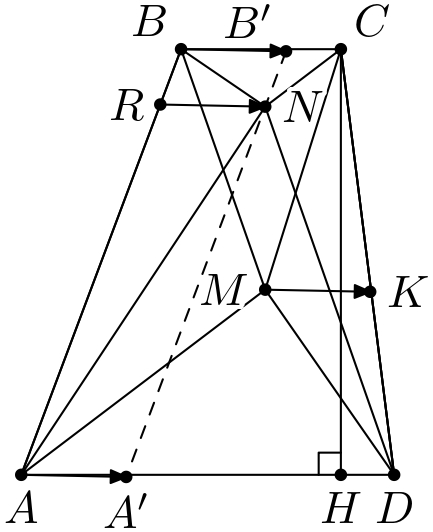
\includegraphics{img_2.jpg} $$

Вернемся к решению задачи. Пусть $R$ и $K$ такие точки, взятые на прямых $BA$ и $CD$ соответственно так, что $RN \parallel BC \parallel MK$. Пусть при параллельном переносе на вектор $\overrightarrow{MK}$ точки $B’$ и $A’$ оказались образами точек $B$ и $A$, соответственно. 

Так как $CN \parallel AM \parallel A’K$ и $DN \parallel BM \parallel B’K$, то $CN \parallel A’K$ и $DN \parallel B'K$. Пусть $CN$ пересекает $B'A'$ в точке $N'$. Так как $A'K \parallel CN'$, то, по лемме, примененной к трапеции $A'B'CD$, $B'K \parallel N'D$. Значит, $DN \parallel B'K \parallel N'D$ и $N' = N$. То есть, точка $N$ лежит на прямой $B’A’$. 

Следовательно,  $\overrightarrow{RN} =\overrightarrow{BB'}=\overrightarrow{MK}$. Пусть $CH$ --- высота треугольника $CDA$. Тогда расстояние между прямыми $BC$ и $DA$ равно $CH$ и
$$
S_{MCD}
=
\frac{1}{2} MK \cdot CD \cdot \sin \angle(MK,CD) 
=
\frac{1}{2} MK \cdot CD \cdot \sin \angle HDC 
=
\frac{1}{2} MK \cdot CH
.
$$
Аналогично, $S_{BAN}=\frac{1}{2}RN \cdot CH$. Так как $MK=RN$, то $S_{MCD}=S_{BAN}$, что и требовалось доказать.

\marking

1. Показано, что $S_{BCD}=S_{BCA}$ или $S_{BAD}=S_{CAD}$: \dotfill\textbf{1~балл}

2. Доказана лемма из решения выше: \dotfill\textbf{2~балла}

\smallskip
3. Доказано равенство $\overrightarrow{RN} =\overrightarrow{MK}$: \dotfill\textbf{3~балла}

\smallskip

\textit{За вычислительное решение (в координатах, в комплексных числах, в векторах, тригонометрическое, и т.д.), не доведённое до конца, можно получить баллы только если результаты промежуточных вычислений сформулированы в виде равносильных геометрических утверждений, указанных в схеме оценки.}


\Problem{2} Дано натуральное $n$. В клетчатом квадрате $2n\times 2n$  каждая клетка покрашена в какой-то из $4n^2$ цветов (при этом некоторые цвета могли не использоваться). \textit{Доминошкой} будем называть любой прямоугольник из двух клеток в нашем квадрате. Будем говорить, что доминошка \textit{разноцветная}, если клетки в ней разных цветов.

Пусть $k$ --- количество разноцветных доминошек среди всех доминошек в нашем квадрате. Пусть $\ell$ --- наибольшее целое число такое, что в любом разрезании квадрата на доминошки найдётся хотя бы $\ell$ разноцветных доминошек. Найдите наибольшее возможное значение выражения $4\ell - k$ по всем возможным раскраскам квадрата. \avtor{Богданов~И.}

\answer $4n$.

\solution Рассмотрим раскраску квадрата, в которой все клетки покрашены в попарно различные цвета. При такой раскраске любая доминошка разноцветная, а значит $k = 2 \cdot 2n \cdot (2n - 1) = 8 n^2 - 4 n$ и $\ell = (2n)^2 / 2 = 2 n^2$. Следовательно, для этой раскраски, $4 \ell - k = 4 n$.

Теперь достаточно доказать, что $4 \ell - k \leq 4n$ для любой раскраски. Рассмотрим четыре разрезания квадрата на доминошки, изображенные на картинке снизу. Разрезания $\mathcal P_1$ и $\mathcal P_2$ состоят только из горизонтальных и только из вертикальных доминошек, соответственно. В разрезании $\mathcal P_3$ самый левый и самый правый столбцы разрезаются на вертикальные доминошки, а оставшаяся часть --- на горизонтальные. Разрезание $\mathcal P_4$ получается из $\mathcal P_3$ поворотом на $90^\circ$. 

\medskip
\centerline{\includegraphics{img_3.mps}}
\medskip

Заметим, что любая доминошка присутствует не более чем в двух из этих четырех разрезаний. Более того, есть ровно $4n$ доминошек, присутствующих в двух разрезаниях --- вертикальные доминошки в $\mathcal P_3$ и горизонтальные в $\mathcal P_4$.

По условию, в каждом из четырех разрезаний, указанных выше, хотя бы $\ell$ разноцветных доминошек. Но разноцветных доминошек всего в квадрате $k$, и максимум $4n$ из них встречаются в двух разрезаниях. Следовательно, $4 \ell \leq k + 4n \implies 4 \ell - k \leq 4n$, что и требовалось.

\marking

1. Приведен пример раскраски, при которой $4 \ell - k = 4n$, и правильно посчитаны $k$ и $\ell$ \dotfill\textbf{1~балл}

2. Доказана оценка $4 \ell - k \leq 4n$: \dotfill\textbf{6~баллов}


\Problem{3} Пусть $p$ --- простое число. Построим ориентированный граф на $p$ вершинах, пронумерованных целыми числами от $0$ до $p - 1$. В графе проводится ребро из вершины $x$ в вершину $y$ тогда и только тогда, когда $y$ равно остатку от деления на $p$ числа $x^2 + 1$. Через $f(p)$ обозначим длину самого длинного ориентированного цикла в этом графе. Докажите, что $f(p)$ может принимать сколь угодно большие значения. \avtor{Зиманов~А.}

\solution Рассмотрим рекуррентную последовательность целых чисел $\{ a_{n} \}_{n = 0}^{\infty}$, заданную как $a_{0} = 0$ и $a_{n + 1} = a_{n}^2 + 1$ для всех $n \geq 0$. Для натурального $x$, через $d(x)$ будем обозначать множество его простых делителей. Пусть множество $S = \bigcup_{n = 1}^{\infty} d(a_n)$, то есть множество всех простых чисел, которые делят хотя бы один положительный элемент последовательности. Докажем, что множество $S$ бесконечно. Для этого нам понадобится следующая лемма:

\Lemma Пусть $n > m$ --- произвольные неотрицательные целые числа. Тогда если существует простое число $p$, делящее $a_n$ и $a_m$, то $p$ также делит $a_{\text{НОД}(n, m)}$, где $\text{НОД}(n, m)$ --- наибольший общий делитель чисел $n$ и $m$.

\proof Так как $a_m \equiv 0 \equiv a_0 \pmod{p}$, то $a_{m + 1} \equiv a_{m}^2 + 1 \equiv 1 \equiv a_{1} \pmod{p}$. Далее, по индукции можно доказать, что для любого неотрицательного целого $k$ будет $a_{m + k} \equiv a_{k} \pmod{p}$. Следовательно, $0 \equiv a_{n} \equiv a_{m + (n - m)} \equiv a_{n - m} \pmod{p}$, то есть $a_{n - m}$ делится на $p$. Но это значит, что мы можем применить алгоритм Евклида к индексам $n$ и $m$ и, в итоге, получить, что $p$ делит $a_{\text{НОД}(n, m)}$.
\qed

\corollary Если $q$ --- произвольное простое число, то $a_{q}$ взаимно просто с каждым из $a_1, a_2, \ldots, a_{q - 1}$, так как для $1 \leq k \leq q - 1$ имеем $\text{НОД}(k, q) = 1$, то есть если простое $p$ делит $a_q$ и $a_k$, то $p$ делит $a_{\text{НОД}(k, q)} = a_1 = 1$, что невозможно.

\medskip

Пусть $p_1 = 2, p_2 = 3, p_3 = 5, \ldots$ --- последовательность всех простых чисел. Тогда все множества $d(a_{p_1}), d(a_{p_2}), d(a_{p_3}), \ldots$ непустые и попарно непересекающиеся, следовательно, множество $S$ бесконечно.

Теперь вернемся к исходной задаче. Зафиксируем произвольное натуральное число $N$. Так как $S$ бесконечно, а множество $\bigcup_{n = 1}^{N} d(a_{n})$ простых делителей только среди первых $N$ положительных элементов  конечно, то существует простое число $p \in S$ такое, что $p$ не делит $a_n$ для всех $1 \leq n \leq N$, но делит $a_M$ для какого-то $M > N$.

Посмотрим на описанный в условии граф для этого простого $p$. Заметим, что переход $a_n \to a_{n + 1}$ соответствует переходу по ребру из вершины $a_n \pmod{p}$ в вершину $a_{n + 1} \pmod{p}$. Так как $a_M \equiv 0 \equiv a_0 \pmod{p}$, то вершина $0$ лежит на каком-то простом цикле в этом графе. Так как ни одно из $a_1, a_2, \ldots, a_N$ не делится на $p$, то длина этого цикла не может быть меньше $N + 1$, то есть $f(p)$ точно не меньше $N + 1$. Раз мы фиксировали произвольное натуральное $N$ и доказали существование простого $p$ такого, что $f(p) > N$, то $f(p)$ может принимать сколь угодно большие значения.

\marking

1. Рассмотрена рекуррентная последовательность целых (не по модулю $p$) чисел $\{ a_n \}$:\dotfill\textbf{1~балл}

2. Задача сведена к доказательству бесконечности множества $S$:\dotfill\textbf{2~балла}

3. Доказана лемма, либо только переход из $n$ и $m$ в $(n - m)$:\dotfill\textbf{2~балла}


\Problem{4} Пусть $\mathcal{M} = \mathbb{Q}[x, y, z]$ --- множество многочленов с рациональными коэффициентами от трех переменных. Докажите, что для любого ненулевого многочлена $P \in \mathcal{M}$ существуют такие ненулевые многочлены $Q, R \in \mathcal{M}$, что
$$
R(x^2 y, y^2 z, z^2 x)
=
P(x, y, z) Q(x, y, z)
.
$$ \avtor{Navid Safaei}

\solution Сначала докажем следующую лемму.

\Lemma Для любого ненулевого $P \in \mathcal{M}$ существует такой ненулевой $R \in \mathcal{M}$, что $R(x^3, y, z)$ делится на $P(x, y, z)$.

\proof Пусть $n = \deg P$ и
$$
P(x, y, z)
=
\sum_{i = 0}^{n}
a_i x^i B_i(y, z)
\quad
(B_i \in \mathbb{Q}[y, z]),
$$
$$
A_j(x, y, z)
=
\sum_{\substack{0 \le i \le n \\ i \equiv j \pmod{3}}}
a_i x^i B_i(y, z)
\quad
(0 \le j \le 2)
.
$$

Рассмотрим многочлен
$$
A_0^3 + A_1^3 + A_2^3 - 3 A_0 A_1 A_2 \not\equiv 0
.
$$
С одной стороны, так как переменная $x$ входит в каждый его одночлен в степени, кратной 3, то для какого-то $R \in \mathcal{M}$ он равен $R(x^3, y, z)$. С другой стороны,
$$
A_0^3 + A_1^3 + A_2^3 - 3 A_0 A_1 A_2 
=
(A_0 + A_1 + A_2)
(A_0^2 + A_1^2 + A_2^2 - A_0 A_1 - A_1 A_2 - A_2 A_0)
=
$$
$$
=
P (A_0^2 + A_1^2 + A_2^2 - A_0 A_1 - A_1 A_2 - A_2 A_0)
,
$$
то есть $R(x^3, y, z)$ делится на $P(x, y, z)$. Лемма доказана.
\qed

\corollary Для любого ненулевого $P \in \mathcal{M}$ и любых целых неотрицательных $k, t, \ell$, существует такой ненулевой $R \in \mathcal{M}$, что $R(x^{3^k}, y^{3^t}, z^{3^\ell})$ делится на $P(x, y, z)$. Это легко доказывается по индукции, применяя лемму при переходе.

\medskip

Вернемся к решению задачи. Следствие из леммы, в частности, говорит о существовании такого $S \in \mathcal{M}$, что $S(x^9, y^9, z^9)$ делится на $P(x, y, z)$. Пусть $n = \deg S$. Рассмотрим многочлен
$$
(xyz)^{6n} S(x^9, y^9, z^9) \not \equiv 0
.
$$
Любой его одночлен имеет вид
$$
\alpha (xyz)^{6n} x^{9a} y^{9b} z^{9c}
=
\alpha 
(xyz)^{6 (n - a - b - c)}
(xyz)^{6 (a + b + c)}
x^{9a} y^{9b} z^{9c}
=
$$
$$
=
\alpha 
(xyz)^{6 (n - a - b - c)}
(xyz)^{6 (a + b + c)}
x^{9a} y^{9b} z^{9c}
=
$$
$$
=
\alpha 
(xyz)^{6 (n - a - b - c)}
(x^2y)^{6a+3b}(y^2z)^{6b+3c}(z^2x)^{6c+3a}
=
$$
$$
=
\alpha
(x^2y)^{6a+3b + 2 (n - a - b - c)}
(y^2z)^{6b+3c + 2 (n - a - b - c)}
(z^2x)^{6c+3a + 2 (n - a - b - c)}
.
$$
Следовательно, существует такой $R \in \mathcal{M}$, что
$$
R(x^2 y, y^2 z, z^2 x)
=
(xyz)^{6n} S(x^9, y^9, z^9)
.
$$
Так как $S(x^9, y^9, z^9)$ делится на $P(x, y, z)$, то и $R(x^2 y, y^2 z, z^2 x)$ делится на $P(x, y, z)$.

\par
\bigskip
\textbf{Комментарий.} Лемму можно доказать и другим способом. Пусть $\omega = e^{\frac{2 \pi i}{3}}$ (первообразный корень из единицы третьей степени) и
$$
H(x, y, z)
=
P(x, y, z) P(\omega x, y, z) P(\omega^2 x, y, z)
.
$$
Так как $\overline{\omega} = \omega^2$, то, для $x, y, z \in \mathbb{R}$, 
$$
\overline{P(\omega x, y, z)}
=
P(\overline{\omega} x, y, z)
=
P(\omega^2 x, y, z)
\implies
$$
$$
\implies
\overline{H(x, y, z)}
=
H(x, y, z)
.
$$
Можно показать, что тогда у $H$ действительные (и рациональные) коэффициенты (оставим это в качестве упражнения). Пусть $m = \deg H$ и
$$
H(x, y, z)
=
\sum_{i = 0}^{m}
h_i x^i C_i(y, z)
\quad
(C_i \in \mathbb{Q}[y, z]),
$$
$$
D_j(x, y, z)
=
\sum_{\substack{0 \le i \le n \\ i \equiv j \pmod{3}}}
h_i x^i C_i(y, z)
\quad
(0 \le j \le 2)
.
$$
Заметим, что
$$
H(x, y, z)
=
H(\omega x, y, z)
=
H(\omega^2 x, y, z)
\implies
$$
$$
\implies
D_0 + D_1 + D_2
=
D_0 + \omega D_1 + \omega^2 D_2
=
D_0 + \omega^2 D_1 + \omega D_2
\implies
$$
$$
\implies
D_1
=
D_2
=
0
\implies
H = D_0
.
$$
Следовательно, для какого-то $R \in \mathcal{M}$,
$$
R(x^3, y, z)
=
H(x, y, z)
.
$$

Пусть 
$$
Q(x, y, z) 
=
P(\omega x, y, z) P(\omega^2 x, y, z)
.
$$
Можно показать, что $Q \in \mathcal{M}$. Так как
$$
R(x^3, y, z)
=
H(x, y, z)
=
P(x, y, z) Q(x, y, z)
,
$$
то $R(x^3, y, z)$ делится на $P(x, y, z)$.

\marking

1. Сформулирована лемма либо частный случай ее следствия (допустимо рассмотрение многочленов от одной переменной): $\dotfill$ \textbf{1 балл}

\smallskip

2. Доказано, что достаточно рассматривать только такие $P$, которые представимы в виде $T(x^9, y^9, z^9)$, $T \in \mathcal{M}$ (в решении выше, например, многочлен $P$ заменялся на многочлен $S(x^9, y^9, z^9)$, который делится на $P$). $\dotfill$ \textbf{5 баллов}

\smallskip

3. Задача решена для таких $P$, которые представимы в виде $T(x^9, y^9, z^9)$, $T \in \mathcal{M}$. $\dotfill$ \textbf{1 балл}

\smallskip

Все пункты суммируются.

\end{document}
